\renewcommand{\thetheorem}{8.\arabic{theorem}}
\setcounter{theorem}{0}
% ---------------------------------------------------------------------------
% Provenance of the prose in this file.
%   % Extractor: <model>   the block below was transcribed from Prof. Biran's
%                          handwritten notes by that model
%   % Creator:   <model>   the block below was written by that model and has no
%                          counterpart in the notes
% A tag holds until the next tag.
%
% This chapter was written before the convention existed, so the prose carries
% no tags except on the blocks added by later passes. Untagged prose is the
% original transcription; the AI-Note at the end records which figures and
% expansions are the transcript's rather than the notes'.
% ---------------------------------------------------------------------------
\usetikzlibrary{positioning}  % Required for node placement like "below=0.5cm of..."
\usetikzlibrary{arrows.meta}  % Required for the sleek ">={stealth}" arrows
\usetikzlibrary{shapes}       % Good to have for advanced node shapes
\setcounter{chapter}{7}

\chapter{Span and Linear Combinations}

\subsection{Preparation}

Let $V$ be a vector space over a field $K$. Let $S \subseteq V$ be a subset (which is not necessarily a linear subspace). We aim to answer two fundamental and closely related questions:
\begin{enumerate}[label=\textbf{(\alph*)}]
    \item What is the \emph{smallest} linear subspace of $V$ that contains $S$?
    \item What structure do we obtain if we consider the subset of $V$ formed by taking all possible linear combinations of elements from $S$?
\end{enumerate}

To formalize the concept of a \qt{smallest} subspace, we must first prove that the intersection of any collection of subspaces remains a subspace.

\begin{lemma}[Intersections of Subspaces]
\label{lem:intersection_of_subspaces}
Let $V$ be a vector space over $K$. Let $\{W_i\}_{i \in I}$ be a collection of linear subspaces $W_i \subseteq V$ of $V$, indexed by an arbitrary set $I$ of indices. Then their intersection
\[
W := \bigcap_{i \in I} W_i
\]
is a linear subspace of $V$.
\end{lemma}

\begin{proof}
First, since every $W_i$ is a subspace, the zero vector $0_V$ is contained in every $W_i$ by \cref{lem:subspace_criterion} \textbf{(a)}. Therefore, $0_V \in \bigcap_{i \in I} W_i = W$.

Next, let $a_1, a_2 \in K$ and $w_1, w_2 \in W$. We must show that
\begin{equation} \label{eq:intersection_goal}
a_1 w_1 + a_2 w_2 \in W.
\end{equation}
Choose an arbitrary index $j \in I$. Since $w_1, w_2 \in \bigcap_{i \in I} W_i$, we in particular have $w_1, w_2 \in W_j$. Because $W_j \subseteq V$ is itself a linear subspace, \cref{lem:subspace_criterion} \textbf{(b)} applies to it and gives
\[
a_1 w_1 + a_2 w_2 \in W_j.
\]
We have proved that $a_1 w_1 + a_2 w_2 \in W_j$ holds for \emph{every} $j \in I$, and therefore,
\[
a_1 w_1 + a_2 w_2 \in \bigcap_{i \in I} W_i = W,
\]
which is what we wanted to prove in \eqref{eq:intersection_goal}. By \cref{lem:subspace_criterion}, $W$ is a linear subspace.
\end{proof}

\subsection{The Span}

\begin{definition}[Span]
\label{def:span}
Let $S \subseteq V$ be a subset. Let
\[
\mathcal{N} := \{W \mid W \subseteq V \text{ is a linear subspace, and } S \subseteq W\}
\]
be the collection of all linear subspaces of $V$ that contain $S$. We define the \newterm{span} of $S$ (in $V$) as
\[
\Sp(S) := \bigcap_{W \in \mathcal{N}} W.
\]
\end{definition}

\begin{definition}[Linear Combination]
\label{def:linear_combination}
Let $n \in \mathbb{N}$, let $a_1, \dots, a_n \in K$ be scalars and let $v_1, \dots, v_n \in V$ be vectors. A \newterm{linear combination} of the vectors $v_1, \dots, v_n$ with coefficients $a_1, \dots, a_n$ is the vector
\[
a_1 v_1 + \dots + a_n v_n \in V \quad \left(\text{or equivalently, } \sum_{i=1}^n a_i v_i\right).
\]
\end{definition}

\begin{importantremark}
\label{rem:finite_sums_only}
In this course, we consider \textbf{only finitely many elements} in the sums of linear combinations. Infinite sums require topological notions of limits and convergence, which fall outside the scope of general vector spaces.
\end{importantremark}

The span deserves its name: it is a subspace, and it is the smallest one containing $S$.

\begin{lemma}[The Span is the Smallest Subspace Containing $S$]
\label{lem:span_is_smallest}
Let $S \subseteq V$ be a subset. Then:
\begin{enumerate}[label=\textbf{(\alph*)}]
    \item $\Sp(S) \subseteq V$ is a linear subspace.
    \item If $W \subseteq V$ is a linear subspace with $S \subseteq W$, then $\Sp(S) \subseteq W$.
\end{enumerate}
In other words, $\Sp(S)$ is a linear subspace of $V$, and moreover, among those subspaces that contain $S$, it is the smallest one.
\end{lemma}

\begin{proof}
Statement \textbf{(a)} is immediate from \cref{lem:intersection_of_subspaces}: by \cref{def:span}, $\Sp(S)$ is an intersection of a collection of linear subspaces of $V$, and any such intersection is again a linear subspace. Note that the collection $\mathcal{N}$ is never empty, since $V$ itself is a subspace of $V$ containing $S$.

For \textbf{(b)}, let $W \subseteq V$ be a linear subspace with $S \subseteq W$. Then $W$ is one of the members of the collection $\mathcal{N}$ over which the intersection in \cref{def:span} is taken. An intersection is contained in each of the sets being intersected, and therefore,
\[
\Sp(S) = \bigcap_{W' \in \mathcal{N}} W' \subseteq W. \qedhere
\]
\end{proof}

The next lemma answers the second of our two opening questions, and shows that the two answers agree.

\begin{lemma}[Span as the Set of Linear Combinations]
\label{lem:span_is_linear_combinations}
Let $\emptyset \ne S \subseteq V$. Then $\Sp(S)$ is exactly the set of all possible linear combinations of vectors from $S$:
\begin{align*}
\Sp(S) &= \{a_1 v_1 + \dots + a_n v_n \mid n \in \mathbb{N}, \; a_i \in K, \; v_i \in S \text{ for all } 1 \le i \le n\} \\
&= \text{the subset of } V \text{ obtained by taking all possible linear combinations of vectors from } S.
\end{align*}
\end{lemma}

\begin{remark}
\label{rem:S_finite_or_infinite}
The set $S$ itself can be finite or infinite. Regardless of the size of $S$, each individual linear combination uses only a finite number of elements from $S$.
\end{remark}

\begin{proof}
Let us denote the set of all linear combinations by
\[
\widetilde{\Sp}(S) := \{a_1 v_1 + \dots + a_n v_n \mid n \in \mathbb{N}, \; a_i \in K, \; v_i \in S \text{ for all } 1 \le i \le n\}.
\]

Before diving into the algebra, let us visualize the logical strategy of the proof. We will establish three facts, which together force $\Sp(S) = \widetilde{\Sp}(S)$:

\begin{center}
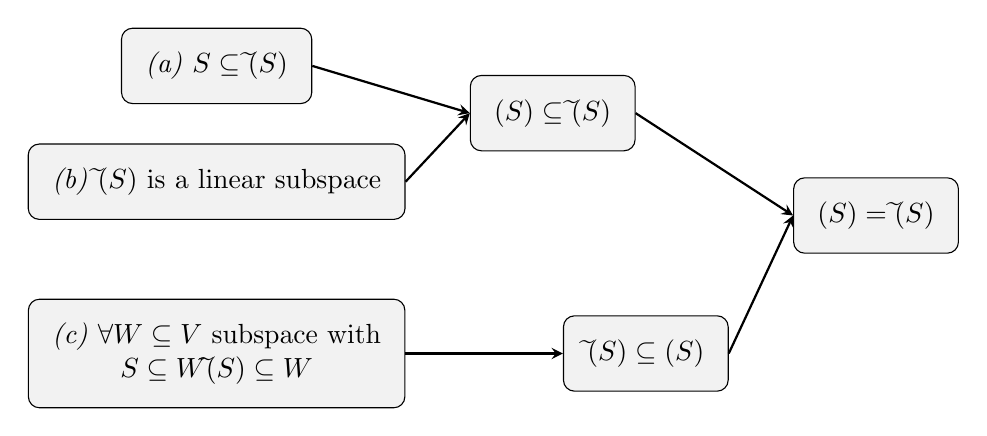
\begin{tikzpicture}[
    node distance=1.5cm and 2cm,
    box/.style={draw, rounded corners, fill=gray!10, align=center, inner sep=2ex},
    arrow/.style={->, thick, >=stealth}
]
    % Left Column (The 3 Facts)
    \node[box] (n1) {\emph{(a)} $S \subseteq \widetilde{\Sp}(S)$};
    \node[box, below=0.5cm of n1] (n2) {\emph{(b)} $\widetilde{\Sp}(S)$ is a linear subspace};
    \node[box, below=1cm of n2] (n3) {\emph{(c)} $\forall W \subseteq V$ subspace with \\ $S \subseteq W \implies \widetilde{\Sp}(S) \subseteq W$};

    % Middle Column (Implications)
    \node[box, right=2cm of n1, yshift=-0.6cm] (p1) {$\Sp(S) \subseteq \widetilde{\Sp}(S)$};
    \node[box, right=2cm of n3] (p2) {$\widetilde{\Sp}(S) \subseteq \Sp(S)$};

    % Right Column (Conclusion)
    \node[box, right=2cm of p1, yshift=-1.3cm] (final) {$\Sp(S) = \widetilde{\Sp}(S)$};

    % Arrows mapping the logic
    \draw[arrow] (n1.east) -- (p1.west);
    \draw[arrow] (n2.east) -- (p1.west);
    \draw[arrow] (n3.east) -- (p2.west);

    \draw[arrow] (p1.east) -- (final.west);
    \draw[arrow] (p2.east) -- (final.west);
\end{tikzpicture}
\end{center}

Note that \textbf{(a)} and \textbf{(b)} imply that $\Sp(S) \subseteq \widetilde{\Sp}(S)$: together they say that $\widetilde{\Sp}(S)$ is one of the subspaces containing $S$, so \cref{lem:span_is_smallest} \textbf{(b)} applies to it. Furthermore, \textbf{(c)} implies that $\widetilde{\Sp}(S) \subseteq \Sp(S)$, because $\Sp(S)$ is itself a subspace $W$ containing $S$ by \cref{lem:span_is_smallest}. Let us now prove the three statements.

\begin{enumerate}[label=\textbf{(\alph*)}]
    \item Let $v \in S$. Then we can write $v = 1 \cdot v \in \widetilde{\Sp}(S)$, which is a linear combination with $n = 1$. Thus, $S \subseteq \widetilde{\Sp}(S)$.

    \item We verify the criterion of \cref{lem:subspace_criterion}. First, $0_V \in \widetilde{\Sp}(S)$: since $S \ne \emptyset$ by assumption, we may pick some $u \in S$, and then $0_V = 0 \cdot u \in \widetilde{\Sp}(S)$ by \cref{lem:vector_space_basics} \textbf{(c)}. \\
    Second, let $v, w \in \widetilde{\Sp}(S)$ and $\alpha, \beta \in K$. Write
    \[
    v = a_1 v_1 + \dots + a_n v_n, \qquad w = b_1 w_1 + \dots + b_m w_m,
    \]
    where $n, m \in \mathbb{N}$, $a_i, b_j \in K$ and $v_i, w_j \in S$ for all $1 \le i \le n$, $1 \le j \le m$. Then
    \[
    \alpha v + \beta w = \alpha a_1 v_1 + \dots + \alpha a_n v_n + \beta b_1 w_1 + \dots + \beta b_m w_m,
    \]
    which is a linear combination of the vectors $v_1, \dots, v_n, w_1, \dots, w_m \in S$ with coefficients $\alpha a_1, \dots, \alpha a_n, \beta b_1, \dots, \beta b_m \in K$. Hence, $\alpha v + \beta w \in \widetilde{\Sp}(S)$, and $\widetilde{\Sp}(S)$ is a linear subspace.

    \item Let $W \subseteq V$ be a linear subspace such that $S \subseteq W$, and let $v \in \widetilde{\Sp}(S)$. We need to show that $v \in W$. Indeed, write $v = a_1 v_1 + \dots + a_n v_n$ for some $n \in \mathbb{N}$, $v_i \in S$ and $a_i \in K$. By assumption $S \subseteq W$, and hence $v_i \in W$ for every $i$. Since $W$ is a linear subspace it is closed under scalar multiplication and under finite sums, and therefore,
    \[
    v = a_1 v_1 + \dots + a_n v_n \in W.
    \]
    Thus $\widetilde{\Sp}(S) \subseteq W$. \qedhere
\end{enumerate}
\end{proof}

\begin{summary}
\label{sum:two_definitions_of_span}
We now have two descriptions of the same object, and we may use whichever is more convenient:
\[
\Sp(S) =
\begin{cases}
\displaystyle \bigcap_{W \in \mathcal{N}} W & \text{(smallest subspace containing } S), \\[2ex]
\text{linear combinations from } S & \text{(by \cref{lem:span_is_linear_combinations}).}
\end{cases}
\]
They can be regarded as equivalent definitions of the span.
\end{summary}

\begin{exercise}[Properties of Span and Subspaces]
\label{exc:span_subspaces_mc}
Let $V$ be a vector space over a field $K$. Which of the following assertions are true?
\begin{enumerate}
    \item For any fixed $v \in V$, the set $W := \{w \in V \mid \exists \lambda \in K : w = \lambda v\}$ is a linear subspace of $V$.
    \item A subset $W \subseteq V$ is a linear subspace if and only if $\Sp(W) = W$.
    \item For any subsets $S_1, S_2 \subseteq V$, we have $\Sp(S_1 \cup S_2) = \Sp(S_1) + \Sp(S_2)$.
    \item For any subsets $S_1, S_2 \subseteq V$, we have $\Sp(S_1 \cap S_2) \subseteq \Sp(S_1) \cap \Sp(S_2)$.
\end{enumerate}
\exinfo{This exercise is Multiple Choice Question 1 of Problem Sheet 7, Linear Algebra I, Autumn Semester 2025.}
\exsol{sol:span_subspaces_mc}
\end{exercise}

\begin{notation}
\label{not:span_of_a_list}
Let $n \in \mathbb{N}$ and $v_1, \dots, v_n \in V$. We write
\[
\Sp(v_1, \dots, v_n) := \Sp(\{v_1, \dots, v_n\}),
\]
dropping the set brackets when the spanning set is given as an explicit finite list.
\end{notation}

\begin{lemma}[The Span of a Finite List]
\label{lem:span_of_finite_list}
Let $n \in \mathbb{N}$ and $v_1, \dots, v_n \in V$. Then
\[
\Sp(v_1, \dots, v_n) = \left\{ \sum_{i=1}^{n} \alpha_i v_i \;\middle|\; \alpha_i \in K \text{ for all } 1 \le i \le n \right\}.
\]
\end{lemma}

\begin{remark}
\label{rem:fixed_number_of_summands}
Note that here the number of summands is fixed at $n$, whereas in \cref{lem:span_is_linear_combinations} it was allowed to vary and the vectors were allowed to repeat. The point is that repetitions and omissions can always be absorbed into the coefficients: a repeated vector has its coefficients added together, and an omitted one is given the coefficient $0$.
\end{remark}

\begin{exercise}[Proof of \cref{lem:span_of_finite_list}]
\label{exc:span_of_finite_list}
Prove \cref{lem:span_of_finite_list}, using \cref{lem:span_is_linear_combinations} together with the observation of the remark above about repetitions and omissions.
\exinfo{This exercise is taken from Prof.~Biran's handwritten lecture notes.}
\exsol{sol:span_of_finite_list}
\end{exercise}

\begin{remark}
\label{rem:span_of_empty_set}
The span of the empty set is the zero subspace:
\[
\Sp(\emptyset) = \{0_V\}.
\]
This is not a convention but a consequence of \cref{def:span}. Every subspace $W \subseteq V$ satisfies $\emptyset \subseteq W$, so the collection $\mathcal{N}$ consists of \emph{all} subspaces of $V$; and since $\{0_V\}$ is one of them, the intersection of all of them is contained in $\{0_V\}$, while $0_V$ lies in every subspace. Using the other description, in terms of linear combinations, we just think of the sum of an empty collection of elements as $0$.
\end{remark}

\subsection{Generating Sets and Finite-Dimensionality}

\begin{definition}[Generating Set]
\label{def:generating_set}
Let $V$ be a vector space over $K$ and let $S \subseteq V$. We say that $S$ \newterm{generates} (or \newterm{spans}) $V$ if
\[
\Sp(S) = V.
\]
In this case $S$ is called a \newterm{generating set} of $V$. More generally, if $\Sp(S) = U$, where $U \subseteq V$ is a subspace of $V$, we say that $S$ generates (or spans) $U$.
\end{definition}

\begin{definition}[Finite-Dimensional Vector Space]
\label{def:finite_dimensional}
A vector space $V$ is called \newterm{finite-di\-men\-sional} if there exists a \emph{finite} set $S \subseteq V$ such that $\Sp(S) = V$. Otherwise, $V$ is called \newterm{infinite-di\-men\-sional}.
\end{definition}

\begin{importantremark}
\label{rem:finite_dim_no_number_yet}
Note that this definition says nothing yet about \emph{how many} vectors a generating set must contain, only that some finite generating set exists. Attaching an actual number to a finite-di\-men\-sional space requires the notion of a basis, and is the business of the next few chapters.
\end{importantremark}

\subsection{The Subspaces of the Plane}

Before turning to computations, let us use the span to list \emph{all} linear subspaces of a small vector space. Take $V := \mathbb{R}^2$ over $K := \mathbb{R}$.

\begin{example}[Lines Through the Origin]
\label{ex:lines_through_origin}
\begin{itemize}
    \item The zero subspace: $\{0_{\mathbb{R}^2}\} = \{(0,0)\} = \Sp(\emptyset) = \Sp(0_{\mathbb{R}^2})$.
    \item Let $0 \ne v = (a,b) \in \mathbb{R}^2$. Then
    \[
    \Sp(v) = \{\alpha \cdot v \mid \alpha \in \mathbb{R}\} = \{(\alpha a, \alpha b) \mid \alpha \in \mathbb{R}\}.
    \]
    Geometrically, this is the line $L_v$ that passes through $(0,0)$ and through $v = (a,b)$, as drawn in \cref{fig:subspaces_of_plane}.
    \item Let $0 \ne v, w \in \mathbb{R}^2$. Then
    \[
    \Sp(v) = \Sp(w)
    \iff \exists \, \alpha \ne 0 \text{ such that } w = \alpha \cdot v
    \iff L_v = L_w.
    \]
\end{itemize}
\end{example}

\begin{figure}[ht!]
  \centering
  \begin{tikzpicture}[scale=1.05, font=\small, >={Stealth[length=2mm]}]
    %, axes ---
    \draw[gray!55, ->] (-2.7,0) -- (2.7,0);
    \draw[gray!55, ->] (0,-2.0) -- (0,2.0);
    %, a family of lines through the origin: the one-dimensional subspaces ---
    \foreach \ang in {20, 62, 108, 152} {
      \draw[ThemeSecondary!40, thin] (\ang:-2.3) -- (\ang:2.3);
    }
    %, the distinguished line L_v ---
    \draw[ThemeAccent, very thick] (30:-2.45) -- (30:2.45);
    \coordinate (V) at (30:2.0);
    %, coordinate drop lines ---
    \draw[gray!80, dashed, thin] (V) -- ($(V)-(0,{2.0*sin(30)})$);
    \draw[gray!80, dashed, thin] (V) -- ($(V)-({2.0*cos(30)},0)$);
    \node[gray, anchor=north, inner sep=2pt, fill=white]
      at ($(V)-(0,{2.0*sin(30)})$) {$a$};
    \node[gray, anchor=east, inner sep=2pt, fill=white]
      at ($(V)-({2.0*cos(30)},0)$) {$b$};
    %, the vector v itself ---
    \fill[ThemePurple] (V) circle (2pt);
    \node[ThemePurple, anchor=south, inner sep=4pt, fill=white]
      at (V) {$v = (a,b)$};
    %, the origin: the zero subspace. The label sits in the widest gap of the
    %     pencil of lines (between 108 and 152 degrees) and masks them locally. ---
    \fill[ThemeGreen] (0,0) circle (2.2pt);
    \node[ThemeGreen!70!black, inner sep=1.5pt, fill=white] at (130:0.8) {$\{0\}$};
    %, the line label goes on the far end, away from v ---
    \node[ThemeAccent, anchor=north east, inner sep=1pt]
      at (30:-2.5) {$L_v = \Sp(v)$};
  \end{tikzpicture}
  \caption{The linear subspaces of $\mathbb{R}^2$. There are exactly three kinds:
  the single point $\{0\}$ (green), the lines through the origin $L_v = \Sp(v)$
  for $0 \ne v$ (one of them highlighted, a few others faint), and $\mathbb{R}^2$
  itself. Two non-zero vectors span the same line precisely when each is a
  non-zero multiple of the other; as soon as $w$ lies off $L_v$, the pair
  $v, w$ already spans the whole plane.}
  \label{fig:subspaces_of_plane}
\end{figure}

\begin{exercise}[Two Vectors Spanning the Same Line]
\label{exc:same_span_same_line}
Prove the two equivalences stated on \cpageref{ex:lines_through_origin}: for $0 \ne v, w \in \mathbb{R}^2$, show that $\Sp(v) = \Sp(w)$ if and only if $w = \alpha \cdot v$ for some $\alpha \ne 0$, and that this holds if and only if $L_v = L_w$.
\exinfo{This exercise is taken from Prof.~Biran's handwritten lecture notes.}
\exsol{sol:same_span_same_line}
\end{exercise}

\begin{exercise}[Two Independent Vectors Span the Plane --- Important!]
\label{exc:two_vectors_span_plane}
Let $W \subseteq \mathbb{R}^2$ be a linear subspace. Suppose $W = \Sp(v, w)$, where $v \ne 0$ and $w \notin \Sp(v)$. Show that $W = \mathbb{R}^2$.
\exinfo{This exercise is taken from Prof.~Biran's handwritten lecture notes.}
\exsol{sol:two_vectors_span_plane}
\end{exercise}

\begin{exercise}[Subspaces and Spans in Two Dimensions]
\label{exc:subspaces_two_dimensions}
Let $v \in \mathbb{R}^2 \setminus \{(0, 0)\}$ and let $w \in \mathbb{R}^2 \setminus \{(0, 0)\}$ be non-zero vectors such that $w \ne \alpha v$ for all $\alpha \in \mathbb{R}$.
\begin{enumerate}
    \item Show that $\Sp(v, w) = \mathbb{R}^2$.
    \item Prove that the only linear subspaces of $\mathbb{R}^2$ are $\{(0, 0)\}$, $\Sp(u)$ for non-zero $u \in \mathbb{R}^2$, and $\mathbb{R}^2$ itself.
\end{enumerate}
\exinfo{This exercise is Problem 2 of Problem Sheet 6, Linear Algebra I, Autumn Semester 2025.}
\exsol{sol:subspaces_two_dimensions}
\end{exercise}

\begin{summary}
\label{sum:subspaces_of_plane}
$\mathbb{R}^2$ has the following linear subspaces, and no others:
\begin{enumerate}[label=\textbf{(\alph*)}]
    \item $\{0_{\mathbb{R}^2}\}$;
    \item $L_v = \Sp(v)$, where $0 \ne v \in \mathbb{R}^2$;
    \item $\mathbb{R}^2$ itself.
\end{enumerate}
\end{summary}

\subsection{Checking for Span: The Bridge to Computations}

Up to this point, our description of the span has been abstract. We now ask a practical, computational question.

\begin{question}
\label{q:membership_in_span}
Let $v_1, \dots, v_n \in K^m$ and $w \in K^m$. How can we determine whether or not $w \in \Sp(v_1, \dots, v_n)$?
\end{question}

For example, take $v_1 := (1,3)$ and $v_2 := (7,73) \in \mathbb{R}^2$, together with $w := (11, 137)$. Here $w$ is indeed in the span, because
\[
-3 \cdot (1,3) + 2 \cdot (7,73) = (-3 + 14, \; -9 + 146) = (11, 137).
\]
But how does one \emph{find} the coefficients $-3$ and $2$? Do they always exist? Are they unique?

\subsubsection{Preparation: a matrix product is a linear combination of columns}

Let
\[
A = \begin{pmatrix}
a_{1,1} & \dots & a_{1,n} \\
\vdots & & \vdots \\
a_{m,1} & \dots & a_{m,n}
\end{pmatrix} \in \M_{m \times n}(K),
\qquad
x = \begin{pmatrix} x_1 \\ \vdots \\ x_n \end{pmatrix} \in K^n,
\]
and let $v_j$ denote the $j$-th column of $A$, that is
\[
v_1 := \begin{pmatrix} a_{1,1} \\ \vdots \\ a_{m,1} \end{pmatrix},
\qquad
v_2 := \begin{pmatrix} a_{1,2} \\ \vdots \\ a_{m,2} \end{pmatrix},
\qquad \dots \qquad
v_n := \begin{pmatrix} a_{1,n} \\ \vdots \\ a_{m,n} \end{pmatrix}
\quad \in K^m,
\]
so that $A$ may be written in column-block form as
\[
A = \begin{pmatrix} | & | & & | \\ v_1 & v_2 & \dots & v_n \\ | & | & & | \end{pmatrix}.
\]
Carrying out the product $A \cdot x$ of \cref{def:matrix_vector_multiplication} and regrouping the terms by columns instead of by rows, we obtain
\begin{equation} \label{eq:product_is_combination}
A \cdot x
= x_1 \begin{pmatrix} | \\ v_1 \\ | \end{pmatrix}
+ x_2 \begin{pmatrix} | \\ v_2 \\ | \end{pmatrix}
+ \dots
+ x_n \begin{pmatrix} | \\ v_n \\ | \end{pmatrix}
= \sum_{i=1}^{n} x_i \cdot v_i.
\end{equation}

This reveals one of the most useful insights in all of linear algebra: \textbf{a matrix-vector product $A \cdot x$ is simply a linear combination of the columns of $A$, weighted by the entries of $x$.} Conversely, we can write any linear combination as a multiplication of a matrix $A$ by a vector $x$.

\subsubsection{The consequence for membership in a span}

So, the problem \qt{find coefficients $x_1, \dots, x_n \in K$ such that $x_1 v_1 + \dots + x_n v_n = w$} is the very same problem as \qt{find a solution $x \in K^n$ of the system $A \cdot x = w$}, where $A$ is the matrix whose columns are $v_1, \dots, v_n$. We record this as a theorem.

\begin{theorem}[Span and Consistency of a Linear System]
\label{thm:span_iff_consistent}
Let $w, v_1, \dots, v_n \in K^m$. Let $A \in \M_{m \times n}(K)$ be the matrix whose columns are exactly the vectors $v_1, \dots, v_n$. Then the target vector $w$ lies in the span of $v_1, \dots, v_n$ if and only if the system of linear equations $A \cdot x = w$ has at least one solution $x = (x_1, \dots, x_n)\transp \in K^n$:
\[
A \cdot x = w \text{ has a solution } x \in K^n
\iff x_1 v_1 + \dots + x_n v_n = w
\iff w \in \Sp(v_1, \dots, v_n).
\]
\end{theorem}

\begin{proof}
The first equivalence is exactly \eqref{eq:product_is_combination}, read from right to left and from left to right. The second is \cref{lem:span_of_finite_list}, which says that the elements of $\Sp(v_1, \dots, v_n)$ are precisely the vectors of the form $\sum_{i=1}^n x_i v_i$ with $x_i \in K$.
\end{proof}

\begin{remark}[How to check this in practice]
\label{rem:span_check_in_practice}
Because of this equivalence, whenever you are asked \qt{is $w$ in the span of these vectors?}, you do not need to guess the coefficients. You simply construct the augmented matrix $(A \mid w)$ and perform Gauss elimination, bringing it to row-reduced echelon form as in \cref{thm:echelon_form_exists}. If the resulting system yields a contradiction, the vector is \textbf{not} in the span. If the system is solvable, the solutions $x_1, \dots, x_n$ are exactly the coefficients needed to build $w$, and by \cref{thm:ero_preserve_solutions}, row reduction has not changed which coefficients those are. Whether the coefficients are \emph{unique} is a separate question, and it is precisely the question of linear independence, which occupies the next chapter.
\end{remark}

\subsection{Some Spaces and How to Generate Them}

To conclude, let us look at some standard vector spaces and identify natural sets of \qt{building block} vectors that span them entirely.

\begin{example}[The Coordinate Space $K^n$]
\label{ex:span_coordinate_space}
Let $V := K^n$ and let
\[
e_1 := (1, 0, \dots, 0), \quad e_2 := (0, 1, 0, \dots, 0), \quad \dots, \quad e_n := (0, \dots, 0, 1)
\]
be the standard vectors. Every vector $(x_1, \dots, x_n) \in K^n$ can be written as $x_1 e_1 + \dots + x_n e_n$, and therefore,
\[
K^n = \Sp(e_1, \dots, e_n).
\]
\end{example}

\begin{exercise}[The Standard Vectors Span $K^n$]
\label{exc:check_standard_span}
Check the identity $K^n = \Sp(e_1, \dots, e_n)$ in detail.
\exinfo{This exercise is taken from Prof.~Biran's handwritten lecture notes.}
\exsol{sol:check_standard_span}
\end{exercise}

\begin{example}[Polynomials]
\label{ex:span_polynomials}
Let $W := K[x]_d$ be the space of polynomials over $K$ of degree $\le d$, introduced as a subspace of $K[x]$ on \cpageref{ex:bounded_degree_subspace}. We can generate this space using the standard monomials:
\[
W = \Sp(1, x, x^2, \dots, x^d).
\]
Let $V := K[x]$ be the space of \emph{all} polynomials over $K$. Generating this space requires an infinite set, since there is no maximum degree:
\[
V = \Sp\bigl(\{1, x, x^2, \dots, x^n, \dots\}\bigr).
\]
\end{example}

\begin{exercise}[Linear Combinations and Span of Polynomials]
\label{exc:polynomial_linear_combination_span}
Consider the following four polynomials in $\mathbb{R}[x]$:
\begin{align*}
p_1(x) &= x^3 + x^2, \\
p_2(x) &= x^2 - 2x - 4, \\
p_3(x) &= 3x + 4, \\
p_4(x) &= 2x + 3.
\end{align*}
\begin{enumerate}
    \item Express the polynomial $q(x) = 2x^3 + 3x^2 - 1$ as an explicit linear combination of $p_1, p_2, p_3, p_4$.
    \item Determine the linear span $\Sp(p_1, p_2, p_3, p_4) \subseteq \mathbb{R}[x]$.
\end{enumerate}
\exinfo{This exercise is Problem 1 of Problem Sheet 6, Linear Algebra I, Autumn Semester 2025.}
\exsol{sol:polynomial_linear_combination_span}
\end{exercise}

\begin{example}[Spaces of Matrices]
\label{ex:span_matrix_space}
Let $\M := \M_{m \times n}(K)$ be the space of all $m \times n$ matrices with entries in $K$. For $1 \le k \le m$ and $1 \le \ell \le n$, let $E_{k\ell} \in \M$ be the matrix that has all its entries $0$ except the entry in position $(k, \ell)$, which is $1$. In other words, $E_{k\ell} = (a_{ij})$, where
\[
a_{ij} =
\begin{cases}
1 & \text{if } i = k \text{ and } j = \ell, \\
0 & \text{otherwise,}
\end{cases}
\qquad \text{so} \qquad
E_{k\ell} =
\begin{pmatrix}
0 & \dots & 0 & \dots & 0 \\
\vdots & & \vdots & & \vdots \\
0 & \dots & 1 & \dots & 0 \\
\vdots & & \vdots & & \vdots \\
0 & \dots & 0 & \dots & 0
\end{pmatrix}
\begin{matrix} \\ \\ \leftarrow \text{row } k \\ \\ \\ \end{matrix}
\]
with the $1$ sitting in column $\ell$. There are exactly $m \cdot n$ such matrices.

For any matrix $A = (a_{ij}) \in \M_{m \times n}(K)$, we can pull it apart into a linear combination in which the scalar weights are simply the matrix entries themselves:
\[
A = \sum_{k=1}^m \sum_{\ell=1}^n a_{k\ell} \cdot E_{k\ell},
\]
and therefore,
\[
\M_{m \times n}(K) = \Sp\bigl(\{E_{k\ell} \mid 1 \le k \le m, \; 1 \le \ell \le n\}\bigr).
\]
For instance, in $\M_{2 \times 2}(K)$ any matrix can be constructed like this:
\[
\begin{pmatrix} a & b \\ c & d \end{pmatrix} = a \begin{pmatrix} 1 & 0 \\ 0 & 0 \end{pmatrix} + b \begin{pmatrix} 0 & 1 \\ 0 & 0 \end{pmatrix} + c \begin{pmatrix} 0 & 0 \\ 1 & 0 \end{pmatrix} + d \begin{pmatrix} 0 & 0 \\ 0 & 1 \end{pmatrix},
\]
so that a matrix may be viewed as a \qt{vector} built out of simpler matrices.
\end{example}

\begin{exercise}[Finite-Dimensionality of the Standard Examples]
\label{exc:finite_dimensional_examples}
Show that $K^n$, $\M_{m \times n}(K)$ and $K[x]_d$ are finite-di\-men\-sional in the sense of \cref{def:finite_dimensional}. What about $K[x]$? Prove your answer.
\exinfo{This exercise is taken from Prof.~Biran's handwritten lecture notes.}
\exsol{sol:finite_dimensional_examples}
\end{exercise}

\begin{exercise}[Subspaces of Matrices Satisfying a Linear Constraint]
\label{exc:matrix_subspace_vector_constraint}
Let $K$ be a field. Fix a vector $x \in K^n$ and a vector $b \in K^m$. Define the subset of matrices
\[
U := \{A \in \M_{m \times n}(K) \mid A \cdot x = b\} \subseteq \M_{m \times n}(K).
\]
For which values of $x \in K^n$ and $b \in K^m$ is $U$ a linear subspace of $\M_{m \times n}(K)$?
\exinfo{This exercise is Problem 4 of Problem Sheet 6, Linear Algebra I, Autumn Semester 2025.}
\exsol{sol:matrix_subspace_vector_constraint}
\end{exercise}

\begin{exercise}[Infinite-Dimensionality of Polynomial Spaces]
\label{exc:polynomial_space_infinite_dim}
Prove that the vector space $K[x]$ of all polynomials over a field $K$ is not finite-dimensional.
\exinfo{This exercise is Problem 5 of Problem Sheet 6, Linear Algebra I, Autumn Semester 2025.}
\exsol{sol:polynomial_space_infinite_dim}
\end{exercise}

\begin{exercise}[Generating Sets for Sequence Spaces]
\label{exc:generating_sets_sequences}
Let $K$ be a field.
\begin{enumerate}
    \item Let $K_0^\infty \subseteq K^\infty$ denote the space of finitely supported sequences:
    \[
    K_0^\infty := \{(a_0, a_1, \dots) \in K^\infty \mid \exists N \ge 0 \text{ such that } a_n = 0 \;\forall n \ge N\}.
    \]
    Find the smallest (with respect to set inclusion) generating subset $E \subseteq K_0^\infty$ and justify your answer.
    \item Let $K_{\mathrm{cst}}^\infty \subseteq K^\infty$ denote the space of eventually constant sequences:
    \[
    K_{\mathrm{cst}}^\infty := \{(a_0, a_1, \dots) \in K^\infty \mid \exists c \in K, \, \exists N \ge 0 \text{ such that } a_n = c \;\forall n \ge N\}.
    \]
    Find the smallest generating subset of $K_{\mathrm{cst}}^\infty$ and justify your answer.
\end{enumerate}
\exinfo{This exercise is Problem 6 of Problem Sheet 6, Linear Algebra I, Autumn Semester 2025.}
\exsol{sol:generating_sets_sequences}
\end{exercise}

\begin{ainote}
The lecture notes write $\Sp(S)$ throughout, which this transcript keeps. The
logical roadmap diagram inside the proof of
\cref{lem:span_is_linear_combinations}, \cref{fig:subspaces_of_plane}, and the
closing sentence about uniqueness in the practical remark on
\cpageref{rem:span_check_in_practice} were added here; everything else follows
the notes. \Cref{lem:span_is_smallest} is
stated in the notes with the proof left as \qt{check the details}, and is proved
in full above.
\end{ainote}

% Creator: Opus 5
\subsection{Solutions to the Exercises}
\label{sec:solutions_span}

\begin{exercisesolution}[Proof of \cref{lem:span_of_finite_list}, which is \cref{exc:span_of_finite_list}]
\label{sol:span_of_finite_list}
Write $S := \{v_1, \dots, v_n\}$ and let $R$ denote the right-hand side of the asserted identity, the set of sums $\sum_{i=1}^n \alpha_i v_i$ with $n$ terms in the fixed order given.

By \cref{lem:span_is_linear_combinations}, $\Sp(S)$ is the set of all linear combinations $\sum_{j=1}^{k} \beta_j u_j$ with $k \ge 0$, $\beta_j \in K$ and $u_j \in S$, where $k$ is not fixed and the $u_j$ need not be distinct. We show the two inclusions.

$R \subseteq \Sp(S)$: a sum $\sum_{i=1}^n \alpha_i v_i$ is already of that form, with $k = n$ and $u_i = v_i$.

$\Sp(S) \subseteq R$: let $\sum_{j=1}^{k} \beta_j u_j$ be given, with each $u_j \in S$. For each $1 \le i \le n$ put
\[
    \alpha_i := \sum_{\substack{1 \le j \le k \\ u_j = v_i}} \beta_j \in K,
\]
the sum over those indices $j$ at which the vector $v_i$ occurs, and $\alpha_i := 0$ if $v_i$ does not occur at all. Regrouping the $k$ summands according to which element of $S$ they involve, which is legitimate by commutativity and associativity of addition in $V$, and collecting the coefficients by distributivity (V7), gives
\[
    \sum_{j=1}^{k} \beta_j u_j = \sum_{i=1}^{n} \alpha_i v_i \in R.
\]
This is exactly the observation of the Remark above: a repeated vector has its coefficients added together, and an omitted one is given the coefficient $0$. The empty combination, $k = 0$, becomes the sum with all $\alpha_i = 0$, which is $0_V$.
\end{exercisesolution}

\begin{exercisesolution}[Proof of \cref{exc:same_span_same_line}]
\label{sol:same_span_same_line}
Let $0 \ne v, w \in \mathbb{R}^2$. We prove the two equivalences in turn.

\textbf{$\Sp(v) = \Sp(w) \iff w = \alpha v$ for some $\alpha \ne 0$.} Suppose the spans agree. Then $w \in \Sp(w) = \Sp(v)$, so $w = \alpha v$ for some $\alpha \in \mathbb{R}$ by \cref{lem:span_of_finite_list}, and $\alpha \ne 0$ because $\alpha = 0$ would give $w = 0$, which is excluded. Conversely, suppose $w = \alpha v$ with $\alpha \ne 0$. Then $w \in \Sp(v)$, and since $\Sp(v)$ is a subspace, $\Sp(w) \subseteq \Sp(v)$ by \cref{lem:span_is_smallest}. Multiplying by $\alpha^{-1}$, which exists because $\alpha \ne 0$, gives $v = \alpha^{-1} w \in \Sp(w)$, and the same argument gives $\Sp(v) \subseteq \Sp(w)$.

\textbf{$w = \alpha v$ for some $\alpha \ne 0 \iff L_v = L_w$.} By the description in \cref{ex:lines_through_origin}, $L_v$ is by definition the set $\{\alpha v \mid \alpha \in \mathbb{R}\} = \Sp(v)$, and likewise $L_w = \Sp(w)$. So, this second equivalence is the first one restated, once the geometric line is identified with the span. That identification is the whole content of the example: \qt{the line through $0$ and $v$} and \qt{the span of $v$} name the same subset of $\mathbb{R}^2$.
\end{exercisesolution}

\begin{exercisesolution}[Proof of \cref{exc:two_vectors_span_plane}]
\label{sol:two_vectors_span_plane}
Let $v = (a, b) \ne 0$ and $w = (c, d) \notin \Sp(v)$, and let $W := \Sp(v, w)$. By \cref{lem:span_of_finite_list}, $W = \{\alpha v + \beta w \mid \alpha, \beta \in \mathbb{R}\}$, so the claim is that every $u = (u_1, u_2) \in \mathbb{R}^2$ can be written in that form.

\textbf{First, $ad - bc \ne 0$.} Suppose instead that $ad = bc$. Since $v \ne 0$, at least one of $a$, $b$ is non-zero; say $a \ne 0$, the case $b \ne 0$ being identical with the two coordinates exchanged. Then $d = \frac{bc}{a}$, and therefore
\[
    w = (c, d) = \left(c, \frac{bc}{a}\right) = \frac{c}{a} \cdot (a, b) = \frac{c}{a} \cdot v \in \Sp(v),
\]
contrary to the hypothesis $w \notin \Sp(v)$.

\textbf{Second, the coefficients exist.} With $\Delta := ad - bc \ne 0$, put
\[
    \alpha := \frac{u_1 d - u_2 c}{\Delta}, \qquad \beta := \frac{u_2 a - u_1 b}{\Delta}.
\]
Then, computing the two coordinates of $\alpha v + \beta w$ separately,
\[
    \alpha a + \beta c = \frac{a u_1 d - a u_2 c + c u_2 a - c u_1 b}{\Delta} = \frac{u_1 (ad - bc)}{\Delta} = u_1,
\]
\[
    \alpha b + \beta d = \frac{b u_1 d - b u_2 c + d u_2 a - d u_1 b}{\Delta} = \frac{u_2 (ad - bc)}{\Delta} = u_2,
\]
so $\alpha v + \beta w = u$. Hence, every $u \in \mathbb{R}^2$ lies in $W$, and $W = \mathbb{R}^2$.

(The quantity $\Delta$ is the determinant of the matrix with columns $v$ and $w$, and the two displayed formulas are Cramer's rule for a $2 \times 2$ system. Neither notion is available yet, and neither is needed: the computation above is self-contained.)

This exercise is marked \qt{Important} for a reason: together with the previous one it is what justifies the word \qt{and no others} in the Summary on \cpageref{sum:subspaces_of_plane}. Given any subspace $W \subseteq \mathbb{R}^2$, either $W = \{0\}$, or it contains some $v \ne 0$ and hence $\Sp(v) \subseteq W$. In the second case either $W = \Sp(v)$, a line, or there is a $w \in W$ outside $\Sp(v)$, and then $\mathbb{R}^2 = \Sp(v,w) \subseteq W$ by what we have just proved. There is no fourth possibility.
\end{exercisesolution}

\begin{exercisesolution}[Proof of \cref{exc:check_standard_span}]
\label{sol:check_standard_span}
Recall $e_i := (0, \dots, 0, 1, 0, \dots, 0) \in K^n$, with the $1$ in position $i$. The inclusion $\Sp(e_1, \dots, e_n) \subseteq K^n$ holds because $\Sp$ of a subset of $K^n$ is a subspace of $K^n$, by \cref{lem:span_is_smallest}.

For the reverse inclusion, let $x = (x_1, \dots, x_n) \in K^n$. Then
\[
    \sum_{i=1}^{n} x_i \, e_i
    = x_1 (1, 0, \dots, 0) + x_2 (0, 1, 0, \dots, 0) + \dots + x_n (0, \dots, 0, 1)
    = (x_1, x_2, \dots, x_n) = x,
\]
where the middle equality is the definition of the operations on $K^n$, applied coordinate by coordinate: coordinate $j$ of the sum is $\sum_i x_i (e_i)_j = x_j$, since $(e_i)_j$ is $1$ for $i = j$ and $0$ otherwise. So, $x \in \Sp(e_1, \dots, e_n)$ by \cref{lem:span_of_finite_list}.

Two things are worth noticing. The coefficients used are the coordinates of $x$ themselves, so they are visibly unique; that uniqueness is what makes $(e_1, \dots, e_n)$ a basis in ch. 10a and $\Phi_{\mathcal{B}}$ well defined in ch. 16. And the computation used nothing about $K$ beyond the field axioms, so it holds over $\mathbb{F}_2$ exactly as over $\mathbb{R}$.
\end{exercisesolution}

\begin{exercisesolution}[Proof of \cref{exc:finite_dimensional_examples}]
\label{sol:finite_dimensional_examples}
By \cref{def:finite_dimensional}, a space is finite-di\-men\-sional when some \emph{finite} subset spans it. Three of the four are, and the fourth is not.

\textbf{$K^n$.} The previous solution exhibits the finite generating set $\{e_1, \dots, e_n\}$, of size $n$.

\textbf{$\M_{m \times n}(K)$.} For $1 \le i \le m$ and $1 \le j \le n$ let $E_{ij}$ be the matrix with $1$ in position $(i,j)$ and $0$ elsewhere. Any $A = (a_{ij})$ satisfies $A = \sum_{i,j} a_{ij} E_{ij}$, since the two sides agree in every entry. So, $\M_{m \times n}(K) = \Sp(\{E_{ij}\})$, a generating set of size $m \cdot n$. This is the computation displayed in \cref{ex:span_matrix_space} above, read as a statement about spanning.

\textbf{$K[x]_d$.} Every $f$ with $\deg f \le d$ is $f = a_0 + a_1 x + \dots + a_d x^d$, which is a linear combination of $1, x, \dots, x^d$. So, $K[x]_d = \Sp(1, x, \dots, x^d)$, a generating set of size $d+1$.

\textbf{$K[x]$ is \emph{not} finite-di\-men\-sional.} Suppose it were, say $K[x] = \Sp(f_1, \dots, f_k)$ for finitely many polynomials $f_i$. Each $f_i$ has a degree, so
\[
    N := \max \{ \deg f_1, \dots, \deg f_k \}
\]
is a well-defined element of $\mathbb{Z}_{\ge 0} \cup \{-\infty\}$, the maximum of a finite set. Every linear combination $\sum_i \alpha_i f_i$ has all coefficients beyond index $N$ equal to zero, hence degree at most $N$, so $\Sp(f_1, \dots, f_k) \subseteq K[x]_N$. But $x^{N+1} \in K[x]$ has degree $N+1 > N$, so $x^{N+1} \notin K[x]_N$, and therefore $\Sp(f_1, \dots, f_k) \ne K[x]$. This contradicts the assumption, so no finite subset spans $K[x]$.

The contrast between the last two is the useful part. Bounding the degree makes the space finite-di\-men\-sional and removing that bound does not, and the reason is precisely that a linear combination is a \emph{finite} sum, the point recorded in the Important Remark on \cpageref{rem:finite_sums_only}. The same mechanism, in the same words, is what \cref{exc:k_infinity_independent} exploits in the next chapter.
\end{exercisesolution}

% Official Solution (Problem Sheet 6, Multiple Choice)
\begin{exercisesolution}[Solution to \cref{exc:span_subspaces_mc}]
\label{sol:span_subspaces_mc}
All four assertions are \textbf{true}. We verify each in turn:

\begin{enumerate}[label=\textbf{(\arabic*)}]
    \item \textbf{True.} The set $W = \{\lambda v \mid \lambda \in K\}$ is precisely the linear span $\Sp(v)$ of the single vector $v$. By \cref{lem:span_is_smallest}, $\Sp(S)$ is a linear subspace for any subset $S \subseteq V$. Directly: $0 = 0 \cdot v \in W$; for $\lambda_1 v, \lambda_2 v \in W$, $\lambda_1 v + \lambda_2 v = (\lambda_1 + \lambda_2) v \in W$; and for $\mu \in K$, $\mu (\lambda v) = (\mu \lambda) v \in W$.

    \item \textbf{True.} If $W \subseteq V$ is a linear subspace, then by (LSS1)--(LSS3) it contains all linear combinations of its elements, so $\Sp(W) \subseteq W$. Since $W \subseteq \Sp(W)$ always holds, we have $\Sp(W) = W$. Conversely, $\Sp(W)$ is always a linear subspace of $V$, so if $W = \Sp(W)$, then $W$ must be a linear subspace.

    \item \textbf{True.} Any vector in $\Sp(S_1 \cup S_2)$ is a finite linear combination $\sum_{i=1}^k \alpha_i u_i + \sum_{j=1}^m \beta_j v_j$ with $u_i \in S_1$ and $v_j \in S_2$. The first sum lies in $\Sp(S_1)$ and the second in $\Sp(S_2)$, so their sum lies in $\Sp(S_1) + \Sp(S_2)$, showing $\Sp(S_1 \cup S_2) \subseteq \Sp(S_1) + \Sp(S_2)$. Conversely, $S_1 \subseteq S_1 \cup S_2 \implies \Sp(S_1) \subseteq \Sp(S_1 \cup S_2)$ and $S_2 \subseteq S_1 \cup S_2 \implies \Sp(S_2) \subseteq \Sp(S_1 \cup S_2)$. Since $\Sp(S_1 \cup S_2)$ is a subspace containing both $\Sp(S_1)$ and $\Sp(S_2)$, it contains their sum $\Sp(S_1) + \Sp(S_2)$.

    \item \textbf{True.} Since $S_1 \cap S_2 \subseteq S_1$, we have $\Sp(S_1 \cap S_2) \subseteq \Sp(S_1)$. Similarly, $S_1 \cap S_2 \subseteq S_2$ implies $\Sp(S_1 \cap S_2) \subseteq \Sp(S_2)$. Therefore, $\Sp(S_1 \cap S_2) \subseteq \Sp(S_1) \cap \Sp(S_2)$.
\end{enumerate}
\exinfo{Official Solution (Problem Sheet 6, Multiple Choice). Verifies subspace span properties and intersection inclusions.}
\end{exercisesolution}

% Official Solution (Problem Sheet 6, Exercise 2)
\begin{exercisesolution}[Solution to \cref{exc:subspaces_two_dimensions}]
\label{sol:subspaces_two_dimensions}
\begin{enumerate}[label=\textbf{(\alph*)}]
    \item \textbf{Proof that $\Sp(v, w) = \mathbb{R}^2$:}
    Let $v = (v_1, v_2) \ne (0, 0)$ and $w = (w_1, w_2) \ne (0, 0)$ with $w \ne \alpha v$ for all $\alpha \in \mathbb{R}$.
    Since $w$ is not a scalar multiple of $v$, the quantity $\Delta := v_1 w_2 - v_2 w_1 \ne 0$. (If $\Delta = 0$, then with $v_1 \ne 0$ we would have $w_2 = \frac{v_2 w_1}{v_1}$, so $w = \frac{w_1}{v_1} v$, a contradiction.)
    
    Given any arbitrary vector $u = (u_1, u_2) \in \mathbb{R}^2$, we seek scalars $c_1, c_2 \in \mathbb{R}$ such that $c_1 v + c_2 w = u$, which in coordinates reads:
    \[
    \begin{cases}
    c_1 v_1 + c_2 w_1 = u_1 \\
    c_1 v_2 + c_2 w_2 = u_2
    \end{cases}
    \]
    Since $\Delta \ne 0$, this $2 \times 2$ system has the unique solution:
    \[
    c_1 = \frac{u_1 w_2 - u_2 w_1}{\Delta}, \qquad c_2 = \frac{v_1 u_2 - v_2 u_1}{\Delta}.
    \]
    Thus $u = c_1 v + c_2 w \in \Sp(v, w)$, proving $\Sp(v, w) = \mathbb{R}^2$.

    \item \textbf{Classification of all Subspaces of $\mathbb{R}^2$:}
    Let $U \subseteq \mathbb{R}^2$ be an arbitrary linear subspace.
    \begin{itemize}
        \item If $U$ contains only the zero vector, then $U = \{(0, 0)\}$.
        \item If $U \ne \{(0, 0)\}$, there exists some non-zero vector $v \in U$. By (LSS3), $\Sp(v) \subseteq U$.
        \begin{itemize}
            \item If $U = \Sp(v)$, then $U$ is a line through the origin.
            \item If $U \ne \Sp(v)$, there exists a vector $w \in U$ such that $w \notin \Sp(v)$. Then $w \ne \alpha v$ for all $\alpha \in \mathbb{R}$. By part \textbf{(a)}, $\Sp(v, w) = \mathbb{R}^2$. Since $v, w \in U$ and $U$ is a subspace, we have $\mathbb{R}^2 = \Sp(v, w) \subseteq U \subseteq \mathbb{R}^2$, which forces $U = \mathbb{R}^2$.
        \end{itemize}
    \end{itemize}
    Thus, the only subspaces of $\mathbb{R}^2$ are $\{(0, 0)\}$, lines through the origin $\Sp(u)$ ($u \ne 0$), and $\mathbb{R}^2$ itself.
\end{enumerate}
\exinfo{Official Solution (Problem Sheet 6, Exercise 2). Proves two non-collinear vectors span $\mathbb{R}^2$ and classifies all subspaces of $\mathbb{R}^2$.}
\end{exercisesolution}

% Solution: Gemini / Official Hybrid (Problem Sheet 6, Exercise 1)
\begin{exercisesolution}[Solution to \cref{exc:polynomial_linear_combination_span}]
\label{sol:polynomial_linear_combination_span}
\begin{enumerate}[label=\textbf{(\alph*)}]
    \item \textbf{Expressing $q(x)$ as a Linear Combination:}
    We seek scalars $\alpha_1, \alpha_2, \alpha_3, \alpha_4 \in \mathbb{R}$ such that
    \[
    \alpha_1 (x^3 + x^2) + \alpha_2 (x^2 - 2x - 4) + \alpha_3 (3x + 4) + \alpha_4 (2x + 3) = 2x^3 + 3x^2 - 1.
    \]
    Equating coefficients of $x^3, x^2, x^1, x^0$:
    \begin{align*}
    [x^3]: & \quad \alpha_1 = 2, \\
    [x^2]: & \quad \alpha_1 + \alpha_2 = 3 \implies 2 + \alpha_2 = 3 \implies \alpha_2 = 1, \\
    [x^1]: & \quad -2\alpha_2 + 3\alpha_3 + 2\alpha_4 = 0 \implies -2(1) + 3\alpha_3 + 2\alpha_4 = 0 \implies 3\alpha_3 + 2\alpha_4 = 2, \\
    [x^0]: & \quad -4\alpha_2 + 4\alpha_3 + 3\alpha_4 = -1 \implies -4(1) + 4\alpha_3 + 3\alpha_4 = -1 \implies 4\alpha_3 + 3\alpha_4 = 3.
    \end{align*}
    Solving the $2 \times 2$ system for $\alpha_3, \alpha_4$:
    \[
    \begin{cases}
    3\alpha_3 + 2\alpha_4 = 2 \\
    4\alpha_3 + 3\alpha_4 = 3
    \end{cases}
    \implies
    \alpha_3 = 3(2) - 2(3) = 0, \quad \alpha_4 = 3(3) - 4(2) = 1.
    \]
    Thus, the linear combination is:
    \[
    q(x) = 2 p_1(x) + 1 p_2(x) + 0 p_3(x) + 1 p_4(x) = 2 p_1(x) + p_2(x) + p_4(x).
    \]

    \item \textbf{Determination of $\Sp(p_1, p_2, p_3, p_4)$:}
    Since each $p_i(x)$ has degree at most $3$, we have $\Sp(p_1, p_2, p_3, p_4) \subseteq \mathbb{R}[x]_3$. We show that the span contains the standard monomial basis $\{1, x, x^2, x^3\}$:
    \begin{itemize}
        \item $3 p_3(x) - 4 p_4(x) = 3(3x + 4) - 4(2x + 3) = x \in \Sp(p_1, p_2, p_3, p_4)$.
        \item $p_3(x) - 3x = 4 \implies 1 = \frac{1}{4}(p_3(x) - 3x) \in \Sp(p_1, p_2, p_3, p_4)$.
        \item $x^2 = p_2(x) + 2x + 4 \in \Sp(p_1, p_2, p_3, p_4)$.
        \item $x^3 = p_1(x) - x^2 \in \Sp(p_1, p_2, p_3, p_4)$.
    \end{itemize}
    Since $\Sp(1, x, x^2, x^3) = \mathbb{R}[x]_3$, we conclude that
    \[
    \Sp(p_1, p_2, p_3, p_4) = \mathbb{R}[x]_3.
    \]
\end{enumerate}
\exinfo{Hybrid Solution (Gemini 3.7 Flash / Official Problem Sheet 6, Exercise 1). Solves the linear system for polynomial coordinates and proves the polynomials span $\mathbb{R}[x]_3$.}
\end{exercisesolution}

% Official Solution (Problem Sheet 6, Exercise 3)
\begin{exercisesolution}[Solution to \cref{exc:matrix_subspace_vector_constraint}]
\label{sol:matrix_subspace_vector_constraint}
The subset $U = \{A \in \M_{m \times n}(K) \mid A \cdot x = b\}$ is a linear subspace of $\M_{m \times n}(K)$ if and only if $b = 0 \in K^m$ (for any $x \in K^n$).

\begin{itemize}
    \item \textbf{Necessity of $b = 0$:}
    If $U$ is a linear subspace, it must contain the zero matrix $0 \in \M_{m \times n}(K)$ by (LSS1). Since $0 \cdot x = 0 \in K^m$ for any vector $x$, the condition $0 \in U$ forces $b = 0 \cdot x = 0$.

    \item \textbf{Sufficiency when $b = 0$:}
    Assume $b = 0$. Then $U = \{A \in \M_{m \times n}(K) \mid A \cdot x = 0\}$. We check the subspace criteria:
    \begin{enumerate}[label=\textbf{(\alph*)}]
        \item The zero matrix satisfies $0 \cdot x = 0$, so $0 \in U$ and $U \ne \emptyset$.
        \item Let $A, B \in U$ and $\alpha, \beta \in K$. Then by the linearity of matrix-vector multiplication (\cref{lem:matrix_vector_linearity}):
        \[
        (\alpha A + \beta B) \cdot x = \alpha (A \cdot x) + \beta (B \cdot x) = \alpha \cdot 0 + \beta \cdot 0 = 0.
        \]
        Thus $\alpha A + \beta B \in U$.
    \end{enumerate}
\end{itemize}
Therefore, $U$ is a linear subspace if and only if $b = 0$.
\exinfo{Official Solution (Problem Sheet 6, Exercise 3). Proves $Ax = b$ subspace criterion requires $b=0$.}
\end{exercisesolution}

% Official Solution (Problem Sheet 6, Exercise 4)
\begin{exercisesolution}[Solution to \cref{exc:polynomial_space_infinite_dim}]
\label{sol:polynomial_space_infinite_dim}
Suppose for contradiction that the vector space $K[x]$ is finite-dimensional. Then by \cref{def:finite_dimensional}, there exists a finite generating set $S = \{f_1, \dots, f_k\} \subset K[x]$ such that $\Sp(S) = K[x]$.

Each polynomial $f_i(x)$ has a well-defined non-negative degree $\deg(f_i)$ (or degree $-\infty$ if $f_i = 0$). Since the set $S$ is finite, the maximum
\[
d := \max_{1 \le i \le k} \deg(f_i) \in \mathbb{Z}_{\ge 0} \cup \{-\infty\}
\]
exists. For any polynomial $g(x) \in \Sp(f_1, \dots, f_k)$, $g(x)$ is a finite linear combination $\sum_{i=1}^k c_i f_i(x)$ with $c_i \in K$. By the properties of polynomial degrees,
\[
\deg(g) \le \max_{1 \le i \le k} \deg(f_i) = d.
\]
Consequently, every element of $\Sp(S)$ has degree at most $d$, so $\Sp(S) \subseteq K[x]_d$.
However, the monomial $x^{d+1}$ belongs to $K[x]$ and has $\deg(x^{d+1}) = d + 1 > d$, so $x^{d+1} \notin \Sp(S)$.
This contradicts the assumption that $\Sp(S) = K[x]$. Therefore, no finite set can span $K[x]$, and $K[x]$ is not finite-dimensional.
\exinfo{Official Solution (Problem Sheet 6, Exercise 4). Demonstrates $K[x]$ is infinite-dimensional via the degree bound.}
\end{exercisesolution}

% Official Solution (Problem Sheet 6, Exercise 5)
\begin{exercisesolution}[Solution to \cref{exc:generating_sets_sequences}]
\label{sol:generating_sets_sequences}
For each $i \in \mathbb{Z}_{\ge 0}$, let $e_i := (0, \dots, 0, 1, 0, \dots) \in K^\infty$ denote the sequence with $1$ in position $i$ and $0$ in all other positions.

\begin{enumerate}[label=\textbf{(\alph*)}]
    \item \textbf{Smallest Generating Set for $K_0^\infty$:}
    Consider the set $E := \{e_i \mid i \ge 0\} \subseteq K_0^\infty$.
    \begin{itemize}
        \item \textbf{$E$ spans $K_0^\infty$:} Any sequence $a = (a_0, a_1, \dots) \in K_0^\infty$ has only finitely many non-zero terms, say $a_n = 0$ for all $n > N$. Then $a = \sum_{i=0}^N a_i e_i$, which is a finite linear combination of elements of $E$. Hence $\Sp(E) = K_0^\infty$.
        \item \textbf{Minimality:} If $E' \subsetneq E$, there exists some index $k \ge 0$ such that $e_k \notin E'$. Any finite linear combination of elements in $E'$ has $k$-th coordinate equal to $0$, because every $e_j \in E'$ ($j \ne k$) has $(e_j)_k = 0$. Hence $e_k \notin \Sp(E')$, so $\Sp(E') \ne K_0^\infty$.
    \end{itemize}
    Thus, $E = \{e_i \mid i \ge 0\}$ is the unique minimal (under inclusion, up to scalar multiples) generating set of $K_0^\infty$.

    \item \textbf{Smallest Generating Set for $K_{\mathrm{cst}}^\infty$:}
    Let $\mathbf{1} := (1, 1, 1, \dots) \in K_{\mathrm{cst}}^\infty$ be the constant sequence of ones. Consider the set $S := \{e_i \mid i \ge 0\} \cup \{\mathbf{1}\} \subseteq K_{\mathrm{cst}}^\infty$.
    \begin{itemize}
        \item \textbf{$S$ spans $K_{\mathrm{cst}}^\infty$:} Let $a = (a_0, a_1, \dots) \in K_{\mathrm{cst}}^\infty$, so there exist $c \in K$ and $N \ge 0$ such that $a_n = c$ for all $n > N$. The sequence $a - c \cdot \mathbf{1}$ has $n$-th entry $0$ for all $n > N$, so $a - c \cdot \mathbf{1} \in K_0^\infty$. Writing $a - c \cdot \mathbf{1} = \sum_{i=0}^N (a_i - c) e_i$, we obtain
        \[
        a = \sum_{i=0}^N (a_i - c) e_i + c \cdot \mathbf{1} \in \Sp(S).
        \]
        Thus $\Sp(S) = K_{\mathrm{cst}}^\infty$.
        \item \textbf{Minimality:}
        \begin{itemize}
            \item If $\mathbf{1}$ is omitted, $\Sp(E) = K_0^\infty \subsetneq K_{\mathrm{cst}}^\infty$, because $\mathbf{1} \notin K_0^\infty$.
            \item If some $e_k$ is omitted from $S$, consider $\Sp(S \setminus \{e_k\})$. Any element in this span has the form $\sum_{j \ne k} \alpha_j e_j + \beta \mathbf{1}$. If this sequence equals $e_k$, its tail entries must be $0$, which forces $\beta = 0$. But with $\beta = 0$, its $k$-th coordinate is $0 \ne 1$. Hence $e_k \notin \Sp(S \setminus \{e_k\})$.
        \end{itemize}
    \end{itemize}
    Thus, $S = \{e_i \mid i \ge 0\} \cup \{\mathbf{1}\}$ is the minimal generating set of $K_{\mathrm{cst}}^\infty$.
\end{enumerate}
\exinfo{Official Solution (Problem Sheet 6, Exercise 5). Constructs minimal generating sets for finite-support and eventually-constant sequence spaces.}
\end{exercisesolution}



